\documentclass[letterpaper]{article}
%\usepackage[pass]{geometry}
\usepackage[utf8]{inputenc}
\usepackage{graphicx} % Required for inserting images
%\usepackage[margin=1.1in]{geometry}
\usepackage[bottom]{footmisc}
\usepackage[top = 1in, bottom = 1in, left = 1in, right = 1in]{geometry}
\usepackage{setspace}
%\usepackage{bookman}
\usepackage{amsmath,amssymb}
\let\oldcite\cite
\renewcommand{\cite}[1]{\textcolor{blue}{\oldcite{#1}}}
\usepackage{lscape}
\usepackage{booktabs,caption}
\usepackage{hyperref}
\usepackage[authordate,backend=biber]{biblatex-chicago}
\usepackage[flushleft]{threeparttable}
\hypersetup{
    colorlinks=true,
    linkcolor=blue,
    filecolor=magenta,
    urlcolor=blue,
    pdftitle={Overleaf Example},
    pdfpagemode=FullScreen,
    }
\renewcommand\thefootnote{\textcolor{red}{\arabic{footnote}}}
\renewcommand\thefigure{\textcolor{blue}{\arabic{figure}}}
\renewbibmacro*{cite:labelyear+extrayear}{%
    \iffieldundef{labelyear}
      {}
      {\printtext[bibhyperref]{\textcolor{blue}{\printfield{labelyear}\printfield{extrayear}}}}%
}
% \usepackage[authoryear]{natbib}
\usepackage[backend=biber, style=authoryear, maxcitenames=2]{biblatex} % Adjust style and options as needed
\renewcommand*{\finalnamedelim}{\addspace\&\space} % Change & to and
\usepackage{subcaption}
\usepackage[edges]{forest}
\usepackage{longtable}
%\usepackage[a6paper,margin=15mm]{geometry}
\usepackage{booktabs}
\usepackage{tabularray}
\usepackage{xcolor}
\usepackage[T1]{fontenc}
\usepackage{babel}
\usepackage{biblatex}
\usepackage{tikz}
\usepackage{changepage}
\usepackage{mathpazo}
\usepackage{subfigure}
\usepackage{comment}
%\usepackage[style=apa]{biblatex}
\newcommand{\email}[1]{\href{mailto:#1}{\texttt{#1}}}
% \newcommand{\customcite}[1]{\citeauthor{#1} (\citeyear{#1})}
\addbibresource{my bib.bib}
%\usepackage[style=apa]{biblatex}

\title{\fontsize{22pt}{0pt}\selectfont
%\textbf{Working Draft }

%\textcolor{blue}{\textit{SRSA 2024 Working Draft}}

In the Eye of the Storm: Understanding Tornado Consequences on U.S. Economic Outcomes}

\author{Bowei Dong\footnote{Department of Economics, University of Oklahoma. \email{boweidon@ou.edu}. I am grateful for the academic assistance provided by OU faculty Tyler Ransom, and data provided by Riley Wilson (Brigham Young University). } \\Department of Economics \\ University of Oklahoma}
}
\date{Apr 2024}
\doublespacing
\begin{document}


\maketitle


 \begin{center}
    

\textcolor{red}{\Large\textit{For ECON 5253 Use. Working Draft.}}
 \end{center}
% \newpage
\
\
\section{Introduction}
Natural disasters can profoundly impact social outcomes, resulting in tragic consequences such as loss of life, destruction of homes, displacement from jobs, and other significant challenges for affected communities. The United States government has a well-established tradition of providing federal assistance in response to natural disasters \parencite[]{FEMA}. 

This research aims to investigate the aftermath of tornadoes in the United States, specifically focusing on the social impacts including migration patterns, changes in median housing prices, fluctuations in unemployment rates, industry share distribution, and other related factors\footnote{This is a working draft, I have not included all outcome variables yet.}. This research draws inspiration from the work of \textcite{bilal2023anticipating}, where the authors explore various outcome variables such as wage, income per capita, population, employment, adjusted and unadjusted investment \parencite{bilal2023anticipating}. Other researchers, like \textcite{gallagher2023weathering}, have studied the effects of severe tornado strikes on household finances and business viability. They observed that migration from heavily damaged areas increases following such events. I plan to analyze migration patterns using various datasets and criteria\footnote{According to \textcite{gallagher2023weathering}, they have used several standards to decide if a tornado should be included: First, the tornado occurs from 2002-2013 so as to match the period covered by our individual and business financial data. Second, the tornado must have a Fujita (F) or Enhanced Fujita (EF) rating of either a 4 or 5.Third,the tornado must have a high quality damage path map,generally created by the NWS, that demarcates areas of the tornado path that suffered different levels of damage.}.

Similarly, several researchers have explored the impacts of Hurricane Katrina in 2005. For instance, \textcite{gallagher2017household} investigated the effects of flooding on household finances and discovered that higher levels of flooding led to more significant reductions in total debt. The study by \textcite{vigdor2008economic} highlights the initial impact of Hurricane Katrina on the population of New Orleans, which involved a near-total evacuation of the city. The hurricane rendered two-thirds of the city's housing stock uninhabitable, at least in the short term. Additionally, Hurricane Katrina resulted in reductions in both the number of workers and the number of firms operating in the city of New Orleans.

This research employs a range of empirical methods, including a two-way fixed effects panel analysis, a gravity model, and a two-way fixed staggered event study. By leveraging combined data sources, I identify the significant influence of tornado severity on migration flows, median housing prices, and labor markets. These findings remain consistent across various model setups and robustness checks, providing valuable insights for urban planners and local economic stakeholders.

Understanding these economic consequences is critical for policymakers, disaster response agencies, and researchers to develop effective strategies for disaster preparedness, response, and recovery. By studying the economic aftermath of natural disasters, we can identify patterns, vulnerabilities, and potential interventions that can mitigate the negative effects and facilitate the restoration and resilience of affected communities over time. 

This work is structured as follows: Section \ref{3} presents a detailed list of the data and the empirical methods employed in this research. Section \ref{4} offers initial results, section \ref{5} concludes.

\section{Data \& Empirical Framework}
\label{3}
\subsection{Data}
This section introduces the data source applied in this research. This research draws on data from diverse sources. The dataset spans from 1992 to 2020.

\subsubsection{SOI Tax Stats - Migration Data}

The Internal Revenue Service (IRS) is a government agency responsible for enforcing and administering the internal revenue laws of the United States. It was established in 1862 and is a bureau of the Department of the Treasury. The primary responsibility of the IRS is to collect taxes from individuals and businesses based on the tax laws and regulations established by Congress \footnote{Internal Revenue Service. (n.d.). About IRS. \url{https://www.irs.gov/aboutirs}}. 

As the main data source of this research, Internal Revenue Service (IRS) - Survey of Income (SOI)  provides aggregate county-level migration information through out each tax year, the information include the county identifier for origins and destinations, number of people flowing from the origins to destinations, number of tax returns received and gross income. Migration data for the United States are based on year-to-year address changes reported on individual income tax returns filed with the IRS. They present migration patterns by State or by county for the entire United States and are available for inflows—the number of new residents who moved to a State or county and where they migrated from, and outflows—the number of residents leaving a State or county and where they went \footnote{This information is collected through Internal Revenue Service (IRS) website, access at \url{https://www.irs.gov/statistics/soi-tax-stats-migration-data}}. 

The IRS SOI Migration data stands out with notable advantages when compared to other migration datasets in the U.S. Firstly, it offers specific information regarding counties and states, catering to diverse requirements within the internal migration literature and facilitating the current research. Secondly, its provision of yearly data is a distinct benefit in contrast to the US Census, which presents migration data on a yearly aggregate basis. Additionally, the IRS data provides a dynamic perspective as it captures the flow from origins to destinations. 

For this study, I employ the dataset spanning from 1992 to 2020. The IRS SOI Migration dataset includes two key migration variables: the "number of returns" and the "number of exemptions." These variables play a crucial role in understanding migration dynamics. The "number of returns" represents the count of individual tax returns filed by households or individuals. It serves as a quantification of the movement of individuals from one location to another, enabling the tracking of migration flows over time. Conversely, the "number of exemptions" signifies the total number of individuals, including both primary taxpayers and their dependents, claimed on tax returns. This measure offers insights into population mobility, considering not only the primary taxpayers but also their accompanying family members. In this study, I utilize the "number of exemptions" variable from the IRS SOI migration data to analyze migration trends and their potential impact on the affected regions.  

\subsubsection{Tornado Data}
Tornado data sourced from NOAA's National Weather Service, specifically the Storm Prediction Center, will be utilized for this research. The study will specifically examine tornado events occurring between 1992 and 2020. By utilizing this dataset, I plot distribution of tornadoes by Enhanced Fajita Scores (EF) in figure (\ref{subfig:locations}) and log formed property loss in figure (\ref{subfig:property_loss}).


\subsubsection{County Distance Database}
County pair distance is included as one of the control variables because various sources indicate that distance is one of the principle factors that drives migration behaviors    (\cite{schwartz1973interpreting}; \cite{bogue1949migration}; \cite{sjaastad1962costs}). This dataset was obtained from the National Bureau of Economic Research (NBER). This variable represents the sole time-invarying factor in this study, acting as a crucial link in the county-to-county migration flow within a gravity model.

\subsubsection{Time-Varying Variables}
The dataset includes county-level disparities, population, gender ratio (calculated as the male population divided by the female population), racial demographics (white and black), and age groups for the years 1990-2020, obtained from the US Census. These variables are essential for building the county-to-county gravity model, as different counties exhibit distinct characteristics that influence migration patterns and other socio-economic dynamics.

Industry shares, including natural resources, construction, manufacturing, and others, are sourced from the Bureau of Labor Statistics. Average weekly wage data is retrieved from the Bureau of Labor Statistics as well.

To establish a consistent comparison of county-level house prices, I utilized a house price index obtained from the Federal Housing Finance Agency (FHFA), which is a developmental index without seasonal adjustments. This index tracks changes in house prices within specific areas but is normalized, limiting direct cross-county comparisons. To create a standardized series for analysis, I gathered 1992-2020 Median housing price data from U.S. Census. \footnote{I want to thank Riley Wilson for helping me obtaining this dataset.}. By applying the house price index to this baseline data, I projected county-level prices backward and forward in time. This process ensured a uniform and comparable series of house price data across counties. Subsequently, I integrated this standardized measure into both the origin and destination county data for each county pair in the analysis. 

2000-2020 Republican and election data are derived from the Harvard Dataverse County Presidential Return.

2000-2020 Civilian labor force and unemployment rate data are obtained from the U.S. Department of Agriculture
(USDA). 

For details, see summary statistics in table (\ref{t0}).


\subsection{Empirical Framework}
This section introduces the models adopted in this research. 
\begin{align}
\label{equ1}
  \large Y_{it} &= \alpha_0 + \alpha_k \sum_{k=1}^{5} \text{Fajita}_{it}^{k} + \alpha_2 \text{Injuries}_{it} + \alpha_3 \text{Fatality}_{it} \nonumber \\
           &\quad + \alpha_4 \text{Property Loss}_{it} + \alpha_5 \text{Crop Loss}_{it} + \alpha_6 \text{N}_{it} + \beta X_{it} + \gamma_i + \lambda_t + \epsilon_{it}
\end{align}


In Equation \ref{equ1}, \( Y_{it} \) represents the dependent variable, which is a measure of migration flows, median housing price at year \( t \) and county \( i \). The model includes explanatory variables such as \( \text{Fajita}_{it}^{k} \), denoting the impact of tornado severity levels (ranging from 1 to 5) on \( Y_{it} \), where \( k \) sums over the tornado severity levels, note that I use max(k)$_{it}$ to represent the scale level in this research. Additionally, \( \text{Injuries}_{it} \), \( \text{Fatality}_{it} \), \( \text{Property Loss}_{it} \), \( \text{Crop Loss}_{it} \), \( \text{N}_{it} \) (potentially representing the number of tornadoes) are included as tornado-related control variables. The coefficients \( \alpha_0, \alpha_k, \alpha_2, \alpha_3, \alpha_4, \alpha_5, \alpha_6, \beta \) capture the effects of these variables on \( Y_{it} \). Furthermore, \( X_{it} \) represents additional covariates affecting \( Y_{it} \), such as demographic characteristics, and \( \gamma_i \) and \( \lambda_t \) denote fixed effects for locations and time periods, respectively. The error term \( \epsilon \) accounts for unobserved factors impacting \( Y_{it} \). This model aims to assess how varying tornado severity levels and related impacts influence the dependent variable, controlling for other factors and fixed effects across locations and time.

\begin{equation}
\label{equ2}
  \large  Y_{odt} =
    \beta Miles_{od} + \Pi'(T_{dt} - T_{ot}) + \Gamma'(X_{dt} - X_{ot}) + \gamma_o + \lambda_d + \phi_t + \epsilon_{odt}
\end{equation}

Equation (\ref{equ2}) draws inspiration from \textcite{wilson2022isolated}, it represents a county-to-county gravity model where tornado-related characteristics are compiled into the variable set \( T \) and control variables into set \( X \). The terms \( \ln(T_{dt} - T_{ot}) \) and \( \ln(X_{dt} - X_{ot}) \) capture county-level disparities between origins (denoted by \( o \)) and destinations (denoted by \( d \)). The outcome variable is the number of exemptions obtained from IRS migration data, serving as a proxy for migration flow from origins to destinations. This model incorporates three fixed effects: origin fixed effects, destination fixed effects, and year fixed effects. The fixed effects help account for unobserved heterogeneity across origins, destinations, and time periods, allowing for a more precise estimation of the impact of tornado-related disparities and control variables on migration flows. Time invarying variable $Miles_{od}$ measures the distance in miles between 2 counties.

\begin{equation}
\label{equ3}
   \large Y_{odt} =
    \Pi'(T_{dt} - T_{ot}) + \Gamma'(X_{dt} - X_{ot}) + \gamma_{od} + \phi_t + \epsilon_{odt}
\end{equation}

Similarly, Equation (\ref{equ3}) adopts origin-to-destination fixed effects and year fixed effects. In this model setup, the distance between origins and destinations (measured in miles) is absorbed by the fixed effects to address collinearity issues. This approach allows the model to focus on the effects of other variables, such as tornado-related disparities and control factors, without the confounding influence of distance, which is implicitly accounted for through the fixed effects.

Equations (\ref{equ1}) through (\ref{equ3}) employ a county-level dynamic panel analysis to assess the overall effects of tornadoes on migration flows (including inflow, outflow, and netflow) and various social indicators such as median housing price, civilian labor force participation, unemployment rate, and the share of Republican voting. The county-level dynamic panel analysis approach offers a convenient way to estimate the aggregate impacts of tornadoes on various social outcomes. However, this method may blur the specific impacts of individual tornadoes and make it challenging to discern the complete mechanism or direct connection between specific tornado events and particular social outcomes. To address this limitation and gain deeper insights into the causal relationships, future research could explore more granular analyses focusing on specific tornado events and their localized effects on social and economic factors, potentially using more sophisticated modeling techniques to disentangle these relationships. Additionally, specific attention is given to tornadoes of relatively severe scales to estimate their impacts on these social outcomes. This analytical approach draws inspiration from \textcite{bilal2023anticipating}, who utilized an event study model to examine the effects of rare climate events (e.g., 1-in-50-years-storms, 1-in-20-years cold waves) on economic activities at the county level, providing insights into the influence of climate change on local economies.

Consider a staggered county-level event study expressed by the equation (\ref{equ4}) (\textcite{sun2021estimating}; \textcite{callaway2021difference}; \textcite{goodman2021difference}):

\begin{equation}
\label{equ4}
\large Y_{it} = \alpha + \sum_{k = T_0}^{T_k} \beta_k \text{treat}_{ik} + \sum_{k = 0}^{T_1} \beta_k \text{treat}_{ik} + X_{it} \Gamma + \phi_i + \gamma_t + \epsilon_{it}
\end{equation}


The regression model described utilizes dummy variables, denoted as \( \text{treat}_{ik} \), which take the value of 1 if the observation's periods relative to the county \( i \)'s first treated period match the value \( k \), and 0 otherwise (and 0 for all never-treated groups). Here, \( T_0 \) and \( T_1 \) represent the lowest and highest number of leads and lags considered surrounding the treatment period, respectively. The controls \( X \) are included to capture additional explanatory factors. The terms \( \phi \) and \( \gamma \) represent county and year fixed effects, respectively. Standard errors are clustered at the county level. $X_{it}$ is the control variable set.

The main objective of this regression is to examine the statistical significance of coefficients on periods before and after treatment. In particular, demonstrating that the coefficients on the pre-treated periods (\( \beta_k \) for \( k < 0 \)) are statistically insignificant supports the parallel trends assumption in Difference-in-Differences (DID) estimation.

In this research, I will focus exclusively on tornadoes classified with a Fajita score of 4 or 5 \parencite{gallagher2023weathering}. The Enhanced Fujita Scale (EF Scale), implemented on February 1, 2007, is utilized to assign a tornado a rating based on estimated wind speeds and associated damage levels (ranging from EF0 to EF5). When assessing tornado-related damage, surveyors compare the damage to a set of Damage Indicators (DIs) and Degrees of Damage (DoD) to estimate the range of wind speeds likely produced by the tornado \parencite[]{NWS}. Tornadoes rated EF4 and EF5 are considered "Devastating" and "Incredible," respectively, with 3-second gust wind speeds ranging from 166 to 200 mph for EF4 and exceeding 200 mph for EF5. I specifically analyze tornado events occurring between 2000 and 2020 in this research, aligning with the data available for analysis during this period. This time frame was chosen based on the availability and reliability of tornado data collected for the study. 

The challenge with conducting a staggered event study focusing on severe tornadoes (EF4 and EF5) arises from certain counties experiencing multiple severe tornado events over the years. For instance, DeKalb County, AL, was impacted by severe tornadoes in 2010 and 2011, while Cleveland County, OK, endured severe tornadoes in 2003, 2010, and 2013. This dataset includes seven counties with recurring severe tornado occurrences. To address this issue, a detailed investigation is conducted for each tornado event to identify and designate the most impacted (the ones with the highest property loss or the highest Fajita score. Cleveland County is an exception as the most severe one was 2013 Moore County tornado\footnote{Information can be found \url{https://en.wikipedia.org/wiki/2013_Moore_tornado}}) as the treated events\footnote{By following this method, following events are selected as treated: 

(1). 2011 DeKalb County, AL \ \ \ (fips 01049) EF5 tornado

(2). 2011 Jackson County, AL\ \ \ \ (fips 01071) EF4 tornado

(3). 2011 Newton County, MO \ (fips 29145) EF5 tornado

(4). 2006 Perry County, MO \ \ \ \ \ \ (fips 29157) EF4 tornado

(5). 2014 Wayne County, NE \ \ \ \ \ (fips 31179) EF4 tornado

(6). 2013 Cleveland County, OK (fips 40027) EF4 tornado

(7). 2008 Madison County, TN \ \ \ (fips 47113) EF4 tornado
}. This approach ensures that the staggered event study captures the most impactful tornado occurrences for analysis.

The robustness check is adopted utilizing \textcite{sun2021estimating}, the results can be found in the appendix.

\section{Initial Results}
\label{4}
\subsection{Overall Impacts of Tornadoes}
First, I present the results of TWFE OLS analysis for migration flows, as shown in Table (\ref{t1}). The outcome variables include inflow, outflow, netflow, which is calculated as inflow minus outflow, and gross flow, which is the summation of inflow and outflow. Columns (1), (3), (5), (7) incorporate control variables such as population, gender gaps, and among others. 

Notably, outflow exhibits a significant decrease associated with milder tornadoes, with the highest coefficient of approximately -0.0186, indicating that when tornadoes are mild, less people are leaving. Gross flow decreases as well, indicating that regions fit by mild tornadoes reduce the active level regarding migration in affected regions.

Table (\ref{t2}) examines the impacts of tornadoes on median housing prices (Columns 1 and 2), civilian labor force (Columns 3 and 4), unemployment rate (Columns 5 and 6), and Republican party votes (Columns 7 and 8). The results indicate that housing prices increase in response to severe tornadoes, with a significant positive coefficient of 1.53\% to 4.14\%. This can be explained through several underlying channels. Firstly, severe tornadoes (e.g., F4 or F5) often cause extensive damage, leading to significant reconstruction efforts and investments in rebuilding damaged properties over time, which can drive up housing prices. Additionally, properties in areas prone to severe tornadoes may require more comprehensive insurance coverage, instilling confidence and increasing perceived safety, thereby boosting property values. Furthermore, major tornado events can prompt shifts in population and housing demand, with affected residents seeking alternative housing options and potentially driving up prices in less-affected or safer nearby areas. 

Table (\ref{t3}) examines the migration flow from origins to destinations, focusing on county-level disparities. The results indicate that migration flow decreases as distance between counties increases. When controlling for origin-to-destination fixed effects (column (2) and (4)), we observe that if the destination county experiences more frequent tornadoes compared to the origin county, migration flow decreases by 0.23, though this effect is minimal.

After tornadoes, various industries are impacted. Table (\ref{t6}) and (\ref{t7}) present the results regarding employment and weekly wage, manufacturing employment increases by 24.8\% following an EF4 tornado, finance workers employment increases with mild tornadoes, trade and transportation employment decreases due to the damage caused by tornadoes, professional and business services workers increases greatly with EF4 tornadoes, by approximately 26.22\%.

When it comes to weekly wage, manufacturing wage increases by 27.1\% and 32.4\% with EF4 and EF5 tornadoes respectively. Finance workers' wage increases by 6\% with EF2 and EF3 tornadoes, professional and business services workers' wage increases by 27.8\% with EF4 tornadoes.

\subsection{Impacts of Severe Tornadoes}

This section presents the findings from the staggered two-way fixed effects (TWFE) event study. The results are depicted in figures and can also be referenced in tables \ref{t4} to \ref{tab9}.


In the aftermath of a tornado, there are noticeable changes in various sectors. For instance, the inflow increases by 3.83\% to 4.16\% one year after the tornado. This increase becomes more pronounced two years after the tornado, with inflow showing a higher increase of 7.11\% to 7.27\%. By the third year, the inflow reaches its peak with an increase of approximately 10.35%.

In the year the tornado occurs, the outflow also increases, ranging from 4.06\% to 4.30\%. This trend continues, and three years after the tornado, the outflow increases further by 6.64\% to 7.01\%.

The housing market also reacts to these changes. One year after the tornado, housing prices increase by 1.20\% to 1.60\%, maintaining stability over the following three years.

However, not all sectors experience growth. Natural resources employment decreases by 6.28\% after the third year following an EF4 tornado and decreases further by 5.7\% in the fifth year. Similarly, employment in the hospitality \& leisure and education \& healthcare sectors decreases by about 3.4\%.

On the other hand, some sectors like finance and professional and business services see an increase in wages. This shows the varied impact of a tornado on different sectors of the economy.


\section{Conclusion}
\label{5}

Natural disasters, such as tornadoes, have widespread consequences including loss of life, property damage, and food insecurity on a global scale. There has been a rapid expansion of literature exploring the relationship between natural disasters and economic activities. 

This study focuses on investigating the effects of tornadoes on several key outcome variables: migration flows (inflow, outflow, netflow, and gross flow), median housing prices, labor market dynamics (civilian labor force participation and unemployment rate), and political inclinations, particularly Republican voting patterns. By analyzing these impacts, this research aims to contribute to the growing body of knowledge concerning the economic and social ramifications of tornadoes, shedding light on their influence across various dimensions of community life and decision-making.

I utilize two-way fixed effects dynamic panel analysis and a two-way fixed effects staggered event study design, leveraging data from sources such as the IRS and U.S. Census, among others, to comprehensively investigate the genuine impacts of tornadoes. This approach allows for a detailed exploration of how tornadoes affect various economic and social indicators, considering both temporal and spatial dimensions through rigorous statistical methods.

The findings from this analysis reveal intriguing patterns related to tornado impacts across different intensity levels. With relatively milder tornadoes (EF0-EF3), outflow is observed to decrease, indicating that fewer people are leaving the affected areas. This could be due to various reasons such as improved conditions or increased opportunities post-disaster. The gross flow also shows a downward trend, suggesting that the regions become less active with mild tornadoes. This could be due to the disruption caused by the tornadoes, leading to a slowdown in activities. Interestingly, more workers seem to engage in the financial industry post-tornado. This could be due to the increased demand for financial services in the aftermath of the disaster. Employment in the professional and business services sector shows an upward trend, indicating a growth in these sectors. This could be due to the need for professional services for rebuilding and recovery efforts. However, employment in the trade and transportation sectors shows a decrease. This could be due to the disruption of trade routes and transportation infrastructure caused by the tornadoes. It highlights the varied impact of tornadoes on different sectors of the economy. The housing prices are observed to increase post-tornado. This could be due to a variety of factors such as increased demand for housing or reduced supply due to the destruction caused by the tornado. In the manufacturing sector, both employment and weekly wages show an upward trend. This suggests that the manufacturing industry may be experiencing growth or recovery following the tornado. The increase in wages could be due to increased demand for manufacturing jobs or improved economic conditions. Similarly, the professional business services sector also shows positive trends. Both employment and wages in this sector are on the rise. This could be due to the increased need for professional services in the aftermath of the tornado, leading to more job opportunities and higher wages in this sector. It highlights the resilience and adaptability of these sectors in the face of natural disasters.

However, this research has several limitations that should be acknowledged. For details, see table (\ref{issue}). These limitations provide opportunities for future research to delve deeper into the complexities of tornado impacts and associated factors.

\pagebreak
\printbibliography

\newpage



\newpage



\newpage
\section*{Appendix A}


\begin{table}[H]
    \centering
    \caption{Summary Statistics}
    \label{t0}
     \resizebox{0.9\textwidth}{!}{%
    \begin{tabular}{l S[table-format=8.4] S[table-format=8.4] S[table-format=8.4] S[table-format=8.4] S[table-format=5.0]}
       \tabularnewline \midrule \midrule
        Variable & Min & Max & Mean & St.D. & N \\
        \midrule
        \multicolumn{6}{l}{\textit{Outcome Variables}} \\
       
        Inflow   & 0.00 & 219429.00 & 3394.80 & 9828.20 & 84,220 \\
        Outflow   & 10.00 & 327776.00 & 3395.55 & 10989.85 & 84,220 \\
        Netflow   & -175818.00 & 108961.00 & -0.74 & 3102.05 & 84,220 \\
        Median Housing Price  & 26519.56 & 4150504.00 & 116545.50 & 84404.76 & 65,681 \\
        Employment \\
        \ \ \ \ \ \ Natural Resources and Mining  & 0.00 & 94792.00 & 597.97 & 2640.92 & 60,075 \\
        \ \ \ \ \ \ Construction  & 0.00 & 176196.00 & 2153.99 & 7208.74 & 60,075 \\
        \ \ \ \ \ \ Manufacturing  & 0.00 & 615501.00 & 4454.34 & 13971.32 & 60,075 \\
         \ \ \ \ \ \ Trade and Transportation  & 0.00 & 842466.00 & 8509.50 & 28742.58 & 60,075 \\
          \ \ \ \ \ \ Information  & 0.00 & 227712.00 & 954.68 & 5871.34 & 60,075 \\
           \ \ \ \ \ \ Financial Activities  & 0.00 & 403774.00 & 2575.13 & 12187.34 & 60,075 \\
           \ \ \ \ \ \ Professional and Business Services  & 0.00 & 638903.00 & 5738.93 & 25770.62 & 60,075 \\
           \ \ \ \ \ \ Education and Healthcare  & 0.00 & 830724.00 & 6240.73 & 22123.31 & 60,075 \\
           \ \ \ \ \ \ Leisure and Hospitality  & 0.00 & 545711.00 & 4584.96 & 16382.51 & 60,075 \\
        Weekly Wage \\
        \ \ \ \ \ \ Natural Resources and Mining  & 0.00 & 5559.00 & 656.36 & 379.49 & 60,075 \\
        \ \ \ \ \ \ Construction  & 0.00 & 3471.00  & 680.77 & 305.26 & 60,075 \\
        \ \ \ \ \ \ Manufacturing  & 0.00 & 6067.00 & 751.74 & 356.50 & 60,075 \\
         \ \ \ \ \ \ Trade and Transportation  & 0.00 & 3927.00 & 579.46 & 171.49 & 60,075 \\
         \ \ \ \ \ \ Information  & 0.00 & 7558.00 & 630.47 & 430.10 & 60,075 \\
         \ \ \ \ \ \ Financial Activities  & 0.00 & 5469.00 & 734.35 & 318.66 & 60,075 \\
          \ \ \ \ \ \ Professional and Business Services  & 0.00 & 10407.00 & 675.56 & 328.82 & 60,075 \\
           \ \ \ \ \ \ Education and Healthcare  & 0.00 & 2462.00 & 591.11 & 201.48 & 60,075 \\
           \ \ \ \ \ \ Leisure and Hospitality  & 0.00 & 1159.00 & 247.58 & 92.06 & 60,075 \\
        & & & & & &\\
        \multicolumn{6}{l}{\textit{Tornado-related Variables}} \\
         
        Enhanced Fujita Score (EF) & 0.00 & 5.00 & 0.17 & 0.53 & 84,220 \\
        Injuries  & 0.00 & 1550.00 & 0.34 & 8.45 & 84,220 \\
        Fatalities  & 0.00 & 158.00 & 0.02 & 0.78 & 84,220 \\
        Property Loss & 0.00 & 1960040000.00 & 56560.32 & 7203459.00 & 84,220 \\
        Crop Loss  & 0.00 & 7500000.00 & 338.79 & 29571.68 & 84,220 \\
        Count of Tornado & 0.00 & 23.00 & 0.39 & 0.95 & 84,220 \\
        & & & & & &\\
        \multicolumn{6}{l}{\textit{Demographic Variables}} \\
        
        Population  & 438.00 & 10094865.00 & 99115.31 & 311354.10 & 84,220 \\
        Gender Gap & 74.30 & 280.01 & 99.26 & 9.83 & 84,220 \\
        White (\%) & 2.61 & 100.00 & 86.30 & 16.23 & 84,220 \\
        Black (\%) & 0.00 & 86.90 & 9.37 & 14.69 & 84,220 \\
        \midrule \midrule
    \end{tabular}}
\end{table}

\begin{table}[H]
    \centering
    
    \caption{Impact of Tornado: Migration}
    \label{t1}
    \small
\begin{tabular}{lcccccccc}
   \tabularnewline \midrule \midrule
   Dependent Variables: & \multicolumn{2}{c}{Inflow} & \multicolumn{2}{c}{Outflow} & \multicolumn{2}{c}{Net Flow} & \multicolumn{2}{c}{Gross Flow}\\
   Average Base Value: & \multicolumn{2}{c}{(3136.22)} & \multicolumn{2}{c}{(3160.06)} & \multicolumn{2}{c}{(-23.83)} & \multicolumn{2}{c}{(6296.28)}\\ 
   Model:          & (1)                    & (2)                    & (3)                    & (4)                     & (5)          & (6)             & (7)                     & (8)\\  
   \midrule
   \emph{Variables}\\
   EF0 (65-85 mph) & -0.0023                & -0.0029                & -0.0075$^{**}$         & -0.0080$^{**}$          & 0.0149       & 0.0163          & -0.0062$^{*}$           & -0.0066$^{**}$\\   
                   & (0.0074)               & (0.0073)               & (0.0037)               & (0.0034)                & (0.0194)     & (0.0193)        & (0.0036)                & (0.0034)\\   
   EF1 (86-110 mph) & -0.0115                & -0.0109                & -0.0076$^{*}$          & -0.0071$^{*}$           & 0.0084       & 0.0087          & -0.0085$^{**}$          & -0.0081$^{**}$\\   
                   & (0.0080)               & (0.0079)               & (0.0044)               & (0.0040)                & (0.0240)     & (0.0239)        & (0.0043)                & (0.0040)\\   
   EF2 (111-135 mph) & -0.0153                & -0.0121                & -0.0186$^{***}$        & -0.0159$^{***}$         & 0.0259       & 0.0263          & -0.0145$^{**}$          & -0.0120$^{**}$\\   
                   & (0.0127)               & (0.0125)               & (0.0062)               & (0.0055)                & (0.0364)     & (0.0362)        & (0.0064)                & (0.0058)\\   
   EF3 (136-165 mph) & -0.0123                & -0.0115                & -0.0090                & -0.0083                 & 0.0550       & 0.0554          & -0.0044                 & -0.0039\\   
                   & (0.0178)               & (0.0170)               & (0.0102)               & (0.0089)                & (0.0627)     & (0.0623)        & (0.0097)                & (0.0086)\\   
   EF4 (166-200 mph) & -0.0037                & -0.0058                & 0.0063                 & 0.0045                  & -0.0392      & -0.0441         & -0.0017                 & -0.0037\\   
                   & (0.0253)               & (0.0230)               & (0.0158)               & (0.0131)                & (0.1340)     & (0.1329)        & (0.0163)                & (0.0137)\\   
   EF5 (Over 200 mph) & 0.0013                 & -0.0059                & 0.0491                 & 0.0436                  & 0.2340       & 0.2461          & 0.0341                  & 0.0287\\   
                   & (0.0756)               & (0.0565)               & (0.0605)               & (0.0433)                & (0.4203)     & (0.4166)        & (0.0608)                & (0.0421)\\   
   Injuries             & $-0.0000$  & $-0.0000$  & $-0.0000$  & $-0.0000$    & -0.0005      & -0.0006         & $-0.0000$   & $-0.0000$\\    
                   & (0.0001)               & (0.0001)               & (0.0001)               & (0.0000)  & (0.0011)     & (0.0011)        & (0.0000)  & (0.0000)\\    
   Fatalities             & 0.0004                 & 0.0014                 & $-0.0000$  & 0.0009                  & 0.0110$^{*}$ & 0.0117$^{*}$    & 0.0001                  & 0.0010\\   
                   & (0.0014)               & (0.0012)               & (0.0016)               & (0.0010)                & (0.0064)     & (0.0064)        & (0.0013)                & (0.0008)\\   
   Property Loss            & 0.0050$^{***}$         & 0.0038$^{***}$         & 0.0041$^{***}$         & 0.0029$^{***}$          & -0.0051      & -0.0058$^{*}$   & 0.0034$^{***}$          & 0.0024$^{***}$\\   
                   & (0.0015)               & (0.0014)               & (0.0009)               & (0.0007)                & (0.0033)     & (0.0032)        & (0.0009)                & (0.0008)\\   
   Crop Loss           & -0.0044                & 0.0006                 & -0.0038                & 0.0013                  & 0.0095       & 0.0102          & -0.0044                 & 0.0002\\   
                   & (0.0051)               & (0.0051)               & (0.0031)               & (0.0031)                & (0.0126)     & (0.0126)        & (0.0032)                & (0.0032)\\   
   Count           & 0.0027                 & 0.0036                 & 0.0038$^{**}$          & 0.0049$^{***}$          & 0.0039       & 0.0045          & 0.0032$^{*}$            & 0.0043$^{***}$\\   
                   & (0.0034)               & (0.0033)               & (0.0016)               & (0.0014)                & (0.0085)     & (0.0084)        & (0.0017)                & (0.0016)\\   
   \midrule                
   \emph{County-Level Control }          &                     & Yes                    &                     & Yes                     &           & Yes             &                      & Yes\\ 
   \midrule
   \emph{Fixed-effects}\\
   County          & Yes                    & Yes                    & Yes                    & Yes                     & Yes          & Yes             & Yes                     & Yes\\  
   Year            & Yes                    & Yes                    & Yes                    & Yes                     & Yes          & Yes             & Yes                     & Yes\\  
   \midrule
   \emph{Fit statistics}\\
   Observations    & 84,220                 & 84,220                 & 84,220                 & 84,220                  & 41,701       & 41,701          & 84,220                  & 84,220\\  
   R$^2$           & 0.93330                & 0.93598                & 0.97728                & 0.98112                 & 0.74103      & 0.74159         & 0.97975                 & 0.98263\\  
   \midrule \midrule
   \multicolumn{9}{l}{\emph{Clustered (County) standard-errors in parentheses}}\\
   \multicolumn{9}{l}{\emph{Signif. Codes: ***: 0.01, **: 0.05, *: 0.1}}\\
\end{tabular}
\end{table}

%%%%%%%%%%%%%%%%%%%%%%%%%%%%%%%%%%%%%%%%%%%%%%%%%%%%%%%%%%%%%%%%%%%%%%%%

\begin{table}[H]
    \centering
    \caption{Impact of Tornado: Other Social Outcomes}
    \label{t2}
    \small
\begin{tabular}{lcccccccc}
   \tabularnewline \midrule \midrule
   Dependent Variables: & \multicolumn{2}{c}{Housing Price} & \multicolumn{2}{c}{Labor Force} & \multicolumn{2}{c}{Unemployment Rate (\%)} & \multicolumn{2}{c}{Republican Vote (\%)}\\
   Average Base Value: & \multicolumn{2}{c}{(120314.70)} & \multicolumn{2}{c}{(48565.99)} & \multicolumn{2}{c}{(6.18)} & \multicolumn{2}{c}{(57.73)}\\
   Model:          & (1)                      & (2)                           & (3)                           & (4)                             & (5)                          & (6)                            & (7)                           & (8)\\  
   \midrule
   \emph{Variables}\\
   EF0 (65-85 mph) & 0.0008                   & 0.0007                        & 0.0017                        & 0.0007                          & 0.0103                       & 0.0074                         & -0.0293                       & 0.0376\\   
                   & (0.0016)                 & (0.0015)                      & (0.0013)                      & (0.0013)                        & (0.0186)                     & (0.0185)                       & (0.1029)                      & (0.0991)\\   
   EF1 (86-110 mph) & -0.0021                  & -0.0023                       & 0.0005                        & 0.0010                          & 0.0975$^{***}$               & 0.0971$^{***}$                 & -0.1010                       & -0.0989\\   
                   & (0.0018)                 & (0.0017)                      & (0.0016)                      & (0.0015)                        & (0.0217)                     & (0.0216)                       & (0.1345)                      & (0.1286)\\   
   EF2 (111-135 mph) & 0.0049$^{**}$            & 0.0040                        & 0.0029                        & 0.0025                          & 0.1064$^{***}$               & 0.1084$^{***}$                 & -0.3735$^{*}$                 & -0.3623$^{*}$\\   
                   & (0.0025)                 & (0.0024)                      & (0.0025)                      & (0.0024)                        & (0.0328)                     & (0.0327)                       & (0.1991)                      & (0.1931)\\   
   EF3 (136-165 mph) & 0.0064$^{*}$             & 0.0054                        & 0.0065$^{*}$                  & 0.0090$^{***}$                  & 0.2060$^{***}$               & 0.2072$^{***}$                 & -0.1514                       & -0.2085\\   
                   & (0.0037)                 & (0.0036)                      & (0.0035)                      & (0.0033)                        & (0.0545)                     & (0.0541)                       & (0.3072)                      & (0.2972)\\   
   EF4 (166-200 mph) & 0.0153$^{**}$            & 0.0159$^{**}$                 & 0.0046                        & 0.0040                          & -0.1133                      & -0.1103                        & 0.2977                        & 0.3009\\   
                   & (0.0071)                 & (0.0068)                      & (0.0061)                      & (0.0057)                        & (0.1250)                     & (0.1239)                       & (0.4482)                      & (0.4285)\\   
   EF5 (Over 200 mph) & 0.0367$^{**}$            & 0.0414$^{***}$                & 0.0087                        & 0.0069                          & -0.3068                      & -0.3119                        & 2.237                         & 2.817$^{*}$\\   
                   & (0.0170)                 & (0.0150)                      & (0.0202)                      & (0.0203)                        & (0.6353)                     & (0.6351)                       & (1.595)                       & (1.690)\\   
   Injuries             & 0.0001                   & 0.0000          & 0.0000          & 0.0000            & 0.0013                       & 0.0012                         & 0.0019                        & 0.0024\\   
                   & (0.0000)    & (0.0000)        & (0.0000)        & (0.0000)          & (0.0016)                     & (0.0016)                       & (0.0039)                      & (0.0031)\\   
   Fatalities             & -0.0010$^{*}$            & -0.0009$^{*}$                 & 0.0000        & 0.0000            & 0.0024                       & 0.0025                         & -0.0314                       & -0.0331\\   
                   & (0.0006)                 & (0.0006)                      & (0.0004)                      & (0.0004)                        & (0.0122)                     & (0.0121)                       & (0.0432)                      & (0.0376)\\   
   Property Loss            & 0.0000    & 0.0000         & 0.0000**  & -0.0000***  & -0.0000       & -0.0000**  & -0.0000**  & 0.0000\\    
                   & (0.0000)  & (0.0000)       & (0.0000)       & (0.0000)         & (0.0000)      & (0.0000)        & (0.0000)        & (0.0000)\\    
   Crop Loss           & -0.0000       & -0.0000         & -0.0000**  & -0.0000**    & 0.0000**  & 0.0000**    & -0.0000        & -0.0000\\    
                   & (0.0000)   & (0.0000)        & (0.0000)        & (0.0000)          & (0.0000)       & (0.0000)         & (0.0000)        & (0.0000)\\    
   Count           & -0.0025$^{***}$          & -0.0016$^{***}$               & -0.0007                       & -0.0005                         & -0.0157$^{**}$               & -0.0153$^{**}$                 & 0.0439                        & 0.0336\\   
                   & (0.0006)                 & (0.0006)                      & (0.0006)                      & (0.0006)                        & (0.0078)                     & (0.0077)                       & (0.0429)                      & (0.0412)\\   
  \midrule                
   \emph{County-Level Control }          &                     & Yes                    &                     & Yes                     &           & Yes             &                      & Yes\\ 
   \midrule
   \emph{Fixed-effects}\\
   County          & Yes                      & Yes                           & Yes                           & Yes                             & Yes                          & Yes                            & Yes                           & Yes\\  
   Year            & Yes                      & Yes                           & Yes                           & Yes                             & Yes                          & Yes                            & Yes                           & Yes\\  
   \midrule
   \emph{Fit statistics}\\
   Observations    & 65,681                   & 65,681                        & 60,023                        & 60,023                          & 60,023                       & 60,023                         & 59,669                        & 59,669\\  
   R$^2$           & 0.95654                  & 0.95929                       & 0.99709                       & 0.99742                         & 0.83803                      & 0.83912                        & 0.81667                       & 0.82975\\  
   \midrule \midrule
   \multicolumn{9}{l}{\emph{Clustered (County) standard-errors in parentheses}}\\
   \multicolumn{9}{l}{\emph{Signif. Codes: ***: 0.01, **: 0.05, *: 0.1}}\\
\end{tabular}
\end{table}

%%%%%%%%%%%%%%%%%%%%%%%%%%%%%%%%%%%%%%%%%%%%%%%%%%%%%%%%%%%%%%%%%%%%%%%%

\begin{table}[H]
    \centering
    \caption{Impact of Tornado: County-to-County Migration}
    \label{t3}
    \small
\begin{tabular}{lcccc}
   \tabularnewline \midrule \midrule
   Dependent Variable: & \multicolumn{4}{c}{Number of Exemptions}\\

   Average Base Value: & \multicolumn{4}{c}{(139.85)}\\
   
   Model:           & (1)                     & (2)                     & (3)                     & (4)\\  
   \midrule
   \emph{Variables (Difference) }\\
   Distance (Miles)   & -0.3083$^{***}$         &                         & -0.3084$^{***}$         &   \\   
                    & (0.0280)                &                         & (0.0280)                &   \\   
   EF             & 0.0903                  & 0.2106                  & 0.0064                  & 0.1405\\   
                    & (0.2150)                & (0.1356)                & (0.1986)                & (0.1296)\\   
   Injuries             & -0.0053                 & 0.0181                  & -0.0048                 & 0.0183\\   
                    & (0.0385)                & (0.0156)                & (0.0372)                & (0.0155)\\   
   Fatalities              & -0.0121                 & -0.1904                 & 0.0023                  & -0.1772\\   
                    & (0.2874)                & (0.2179)                & (0.2747)                & (0.2154)\\   
   Property Loss            & -0.0000   & -0.0000    & -0.0000   & -0.0000\\    
                    & (0.0000)  & (0.0000)  & (0.0000)  & (0.0000)\\    
   Crop Loss           & -0.0000  & -0.0000   & -0.0000   & -0.0000\\    
                    & (0.0000)  & (0.0000)  & (0.0000)  & (0.0000)\\    
   Count          & -0.0032                 & -0.2274$^{*}$           & -0.0504                 & -0.2512$^{**}$\\   
                    & (0.2260)                & (0.1194)                & (0.2291)                & (0.1277)\\   
   \midrule
   \emph{County-Level Control } &                      &                         & Yes                     & Yes \\
   \midrule
   \emph{Fixed-effects}\\
   County Origin   & Yes                     &                         & Yes                     & \\  
   County Destination   & Yes                     &                         & Yes                     & \\  
   Year             & Yes                     & Yes                     & Yes                     & Yes\\  
   County Pair               &                         & Yes                     &                         & Yes\\  
   \midrule
   \emph{Fit statistics}\\
   Observations     & 2,041,439               & 2,041,439               & 2,041,321               & 2,041,321\\  
   R$^2$            & 0.06666                 & 0.95480                 & 0.06668                 & 0.95481\\  
   
   \midrule \midrule
   \multicolumn{5}{l}{\emph{Signif. Codes: ***: 0.01, **: 0.05, *: 0.1}}\\
\end{tabular}
\end{table}


%%%%%%%%%%%%%%%%%%%%%%%%%%%%%%%%%%%%%%%%%%%%%%%%%%%%%%%%%%%%%%%%%%%%%%%%

\begin{table}[H]
    \centering
    \caption{Impacts of Tornado (EF4, EF5) on Migration Flows}
    \label{t4}
    \small
\begin{tabular}{lcccccccc}
   \midrule \midrule
   Dependent Variables: & \multicolumn{2}{c}{Inflow} & \multicolumn{2}{c}{Outflow} & \multicolumn{2}{c}{Net Flow} & \multicolumn{2}{c}{Gross Flow}\\
   Average Base Value: & \multicolumn{2}{c}{(3392.07)} & \multicolumn{2}{c}{(3392.29)} & \multicolumn{2}{c}{(-0.223)} & \multicolumn{2}{c}{(6784.37)}\\ 
   Model:                                    & (1)             & (2)             & (3)             & (4)             & (5)            & (6) & (7)            & (8)\\  
   \midrule
   \emph{Variables}\\
   Years after Tornado $=$ 0  & 0.0297          & 0.0253          & 0.0406$^{*}$    & 0.0430$^{***}$  & 0.2846*        & 0.1199 & 0.0352** & 0.0354***\\   
    & (0.0203)        & (0.0154)        & (0.0208)        & (0.0160)        & (0.1466)       & (0.1345) & (0.0133) & (0.0133)\\   
   Years after Tornado $=$ 1 & 0.0383$^{*}$    & 0.0416$^{**}$   & 0.0102          & 0.0131          & 0.3105***         & 0.2530* & 0.0218 & 0.0253\\   
   & (0.0185)        & (0.0192)        & (0.0273)        & (0.0195)        & (0.0997)       & (0.1338) &(0.0175) & (0.0165)\\   
   Years after Tornado $=$ 2  & 0.0711$^{*}$    & 0.0727$^{***}$  & 0.0276          & 0.0283          & 0.0985         & 0.0368 & 0.0430 & 0.0444**\\   
   & (0.0352)        & (0.0237)        & (0.0313)        & (0.0257)        & (0.1818)       & (0.1499) & (0.0260) & (0.0182) \\   
   Years after Tornado $=$ 3 & 0.1035$^{**}$   & 0.1013$^{***}$  & 0.0701$^{**}$   & 0.0664$^{***}$  & 0.2868*         & 0.2132 & 0.0745** & 0.0715***\\   
   & (0.0426)        & (0.0269)        & (0.0324)        & (0.0188)        & (0.1510)       & (0.1570) & (0.0306) & (0.0182) \\   
   Years after Tornado $=$ 4 & 0.0966$^{***}$  & 0.0920$^{***}$  & 0.0382          & 0.0387$^{*}$    & 0.0875         & -0.0779  & 0.0514** & 0.0491**\\   
   & (0.0280)        & (0.0277)        & (0.0295)        & (0.0234)        & (0.1628)       & (0.1720) & (0.0243) & (0.0222)\\   
   Years after Tornado $=$ 5  & 0.1024$^{***}$  & 0.1014$^{***}$  & 0.0397$^{*}$    & 0.0410$^{*}$    & 0.2776         & 0.1492 & 0.0535** & 0.0528***\\   
   & (0.0326)        & (0.0267)        & (0.0210)        & (0.0224)        & (0.2413)       & (0.1885) & (0.0193) & (0.0204)\\   
   \midrule
   \emph{Fixed-effects}\\
   County                                    & Yes             & Yes             & Yes             & Yes             & Yes            & Yes & Yes            & Yes\\  
   Year                                      & Yes             & Yes             & Yes             & Yes             & Yes            & Yes & Yes            & Yes\\  
   \midrule
   \emph{Fit statistics}\\
   Observations                              & 59,697          & 59,696          & 59,697          & 59,696 &         28,615 & 28,614 & 59,697         & 59,696\\  
   R$^2$                                     & 0.93301         & 0.93310         & 0.98166         & 0.98173         & 0.75784        & 0.76023 & 0.98266 & 0.98271 \\   
   \midrule \midrule
   \multicolumn{7}{l}{\emph{Signif. Codes: ***: 0.01, **: 0.05, *: 0.1}}\\
   
\end{tabular}
\end{table}

%%%%%%%%%%%%%%%%%%%%%%%%%%%%%%%%%%%%%%%%%%%%%%%%%%%%%%%%%%%%%%%%%%%%%%%%

\begin{table}[H]
    \centering
    \caption{Impacts of Tornado (EF4, EF5) on Other Outcome Variables}
    \label{t5}
    \small
\begin{tabular}{lcccccccc}
   \midrule \midrule
   Dependent Variables: & \multicolumn{2}{c}{Housing Price} & \multicolumn{2}{c}{Labor Force} & \multicolumn{2}{c}{Unemployment Rate (\%)} & \multicolumn{2}{c}{Republican Vote (\%)}\\
   Average Base Value: & \multicolumn{2}{c}{(116620.10)} & \multicolumn{2}{c}{(51661.95)} & \multicolumn{2}{c}{(6.11)} & \multicolumn{2}{c}{(58.16)}\\ 
   Model:                                    & (1)             & (2)             & (3)             & (4)             & (5)             & (6)             & (7)            & (8)\\  
   \midrule
   \emph{Variables}\\
   Years after Tornado $=$ 0  & 0.0102          & 0.0078$^{**}$   & 0.0026          & 0.0028          & -0.0040         & -0.0241         & 0.0965         & 0.1720$^{*}$\\   
                                             & (0.0102)        & (0.0032)        & (0.0052)        & (0.0031)        & (0.2667)        & (0.0587)        & (0.9884)       & (0.0969)\\   
   Years after Tornado $=$ 1  & 0.0160$^{*}$    & 0.0120$^{***}$  & 0.0054          & 0.0053          & 0.0069          & -0.0029         & -0.1589        & -0.0053\\   
                                             & (0.0092)        & (0.0040)        & (0.0058)        & (0.0037)        & (0.2035)        & (0.1111)        & (0.7682)       & (0.1827)\\   
   Years after Tornado $=$ 2  & 0.0150$^{**}$   & 0.0103$^{*}$    & 0.0043          & 0.0045          & -0.0006         & 0.0015          & -0.2521        & -0.1081\\   
                                             & (0.0068)        & (0.0055)        & (0.0062)        & (0.0043)        & (0.1925)        & (0.1622)        & (0.7506)       & (0.2848)\\   
   Years after Tornado $=$ 3  & 0.0154$^{*}$    & 0.0111          & 0.0019          & 0.0019          & 0.2205          & 0.2246          & -0.2522        & -0.1264\\   
                                             & (0.0087)        & (0.0076)        & (0.0061)        & (0.0047)        & (0.1810)        & (0.1758)        & (0.8892)       & (0.4143)\\   
  Years after Tornado $=$ 4  & 0.0104          & 0.0067          & 0.0020          & 0.0025          & 0.3082$^{*}$    & 0.3164$^{*}$    & -0.3386        & -0.2056\\   
                                             & (0.0106)        & (0.0098)        & (0.0071)        & (0.0052)        & (0.1690)        & (0.1784)        & (0.7064)       & (0.4450)\\   
   Years after Tornado $=$ 5  & 0.0071          & 0.0046          & 0.0034          & 0.0042          & 0.2767          & 0.3127$^{*}$    & -0.4246        & -0.3264\\   
                                             & (0.0094)        & (0.0109)        & (0.0071)        & (0.0057)        & (0.1681)        & (0.1825)        & (0.8501)       & (0.6056)\\   
   \midrule
   \emph{Fixed-effects}\\
   County                                    & Yes             & Yes             & Yes             & Yes             & Yes             & Yes             & Yes            & Yes\\  
   Year                                      & Yes             & Yes             & Yes             & Yes             & Yes             & Yes             & Yes            & Yes\\  
   \midrule
   \emph{Fit statistics}\\
   Observations                              & 48,427          & 48,426          & 59,645          & 59,644          & 59,645          & 59,644          & 59,291         & 59,290\\  
   R$^2$                                     & 0.96430         & 0.96448         & 0.99866         & 0.99866         & 0.83933         & 0.84026         & 0.83363        & 0.83449\\  

   \midrule \midrule
   \multicolumn{9}{l}{\emph{Signif. Codes: ***: 0.01, **: 0.05, *: 0.1}}\\
\end{tabular}
\end{table}

%%%%%%%%%%%%%%%%%%%%%%%%%%%%%%%%%%%%%%%%%%%%%%%%%%%%%%%%%%%%%%%%%%%%%%%%

\begin{table}[H]
    \centering
    \caption{Impacts of Tornado (EF4, EF5) on Employment}
    \label{t6}
\centering
\resizebox{1.05\textwidth}{!}{%
\begin{tabular}{lccccccccc}
   \tabularnewline \midrule \midrule
   Employment: & Construction  & Information  & Education  & Manufacturing  & Financial & Hospitality & Natural  & Trade and & Professional \\   
      &   &   & and Health  &   & Activities & and Leisure & Resources & Transportation & and Business \\  
   Model:               & (1)                            & (2)                           & (3)                             & (4)                             & (5)                       & (6)                           & (7)                      & (8)                     & (9)\\  
   \midrule
   \emph{Variables}\\
  
  EF0 (65-85 mph)      & 0.0248                         & 0.0304                        & 0.0054                          & 0.0319                          & 0.0188                    & 0.0078                        & 0.0277                   & -0.0037$^{**}$          & 0.0091\\   
                        & (0.0229)                       & (0.0279)                      & (0.0157)                        & (0.0222)                        & (0.0127)                  & (0.0099)                      & (0.0232)                 & (0.0016)                & (0.0200)\\   
   EF1 (86-110 mph)       & 0.0221                         & 0.0218                        & 0.0040                          & 0.0054                          & 0.0195                    & 0.0224                        & -0.0204                  & -0.0035                 & 0.0083\\   
                        & (0.0271)                       & (0.0349)                      & (0.0186)                        & (0.0249)                        & (0.0151)                  & (0.0137)                      & (0.0292)                 & (0.0022)                & (0.0251)\\   
   EF2 (111-135 mph)      & 0.0353                         & 0.0734                        & 0.0217                          & 0.0307                          & 0.0464$^{**}$             & -0.0111                       & 0.0283                   & 0.0002                  & 0.0682$^{*}$\\   
                        & (0.0438)                       & (0.0536)                      & (0.0225)                        & (0.0368)                        & (0.0213)                  & (0.0181)                      & (0.0432)                 & (0.0034)                & (0.0383)\\   
   EF3 (136-165 mph)       & 0.0265                         & -0.1365                       & -0.0032                         & -0.0182                         & 0.0537$^{*}$              & 0.0365                        & -0.0521                  & -0.0117$^{**}$          & 0.0885\\   
                        & (0.0712)                       & (0.0905)                      & (0.0347)                        & (0.0603)                        & (0.0298)                  & (0.0293)                      & (0.0617)                 & (0.0051)                & (0.0622)\\   
  EF4 (166-200 mph)      & 0.0598                         & -0.0696                       & 0.0705                          & 0.2477$^{***}$                  & 0.0131                    & -0.0776                       & 0.1459                   & 0.0026                  & 0.2622$^{***}$\\   
                        & (0.1366)                       & (0.1835)                      & (0.0520)                        & (0.0861)                        & (0.0578)                  & (0.0784)                      & (0.1282)                 & (0.0081)                & (0.0818)\\   
   EF5 (Over 200 mph)      & 0.2975                         & 0.0377                        & 0.0962                          & 0.2492                          & 0.1324                    & 0.0993                        & 0.0211                   & -0.0022                 & -0.4258\\   
                        & (0.2565)                       & (0.3703)                      & (0.0988)                        & (0.2016)                        & (0.0839)                  & (0.0781)                      & (0.1971)                 & (0.0361)                & (0.7389)\\   
   Injuries                  & 0.0002                         & 0.0021$^{**}$                 & -0.0002                         & 0.0007                          & 0.0002                    & -0.0003                       & -0.0005                  & 0.0000    & -0.0010\\   
                        & (0.0007)                       & (0.0009)                      & (0.0002)                        & (0.0005)                        & (0.0006)                  & (0.0003)                      & (0.0007)                 & (0.0000)  & (0.0007)\\   
   Fatalities                  & -0.0030                        & -0.0150$^{*}$                 & 0.0007                          & -0.0112$^{**}$                  & -0.0038                   & -0.0003                       & 0.0032                   & -0.0013$^{*}$           & 0.0078\\   
                        & (0.0087)                       & (0.0090)                      & (0.0030)                        & (0.0054)                        & (0.0054)                  & (0.0031)                      & (0.0090)                 & (0.0007)                & (0.0102)\\   
   Property Loss                 & -0.0074$^{**}$                 & -0.0131$^{***}$               & -0.0029$^{*}$                   & -0.0151$^{***}$                 & -0.0055$^{***}$           & 0.0006                        & -0.0113$^{***}$          & 0.0008                  & -0.0052$^{*}$\\   
                        & (0.0037)                       & (0.0045)                      & (0.0016)                        & (0.0026)                        & (0.0021)                  & (0.0014)                      & (0.0035)                 & (0.0005)                & (0.0030)\\   
   Crop Loss                & -0.0169                        & -0.0041                       & -0.0005                         & 0.0106                          & 0.0134$^{*}$              & -0.0020                       & 0.0028                   & -0.0013                 & -0.0246$^{***}$\\   
                        & (0.0103)                       & (0.0132)                      & (0.0048)                        & (0.0108)                        & (0.0075)                  & (0.0065)                      & (0.0106)                 & (0.0012)                & (0.0076)\\   
   Count                & -0.0050                        & -0.0018                       & -0.0004                         & -0.0069                         & -0.0072                   & 0.0058                        & 0.0025                   & 0.0004                  & -0.0119\\   
                        & (0.0088)                       & (0.0118)                      & (0.0091)                        & (0.0095)                        & (0.0045)                  & (0.0040)                      & (0.0113)                 & (0.0007)                & (0.0078)\\   
   \midrule
   \emph{Fixed-effects}\\
   County               & Yes                            & Yes                           & Yes                             & Yes                             & Yes                       & Yes                           & Yes                      & Yes                     & Yes\\  
   Year                 & Yes                            & Yes                           & Yes                             & Yes                             & Yes                       & Yes                           & Yes                      & Yes                     & Yes\\  
   \midrule
   \emph{Fit statistics}\\
   Observations         & 79,876                         & 75,227                        & 83,216                          & 80,151                          & 82,690                    & 83,582                        & 80,070                   & 84,182                  & 81,922\\  
   R$^2$                & 0.72753                        & 0.80230                       & 0.85747                         & 0.81835                         & 0.79320                   & 0.87653                       & 0.72571                  & 0.99329                 & 0.78908\\  
  
   \midrule \midrule
   \multicolumn{10}{l}{\emph{Clustered (County) standard-errors in parentheses}}\\
   \multicolumn{10}{l}{\emph{Signif. Codes: ***: 0.01, **: 0.05, *: 0.1}}\\
\end{tabular}}
\end{table}

%%%%%%%%%%%%%%%%%%%%%%%%%%%%%%%%%%%%%%%%%%%%%%%%%%%%%%%%%%%%%%%%



\begin{table}[H]
    \centering
    \caption{Impacts of Tornado (EF4, EF5) on Wage}
    \label{t7}
\centering
\resizebox{1.05\textwidth}{!}{%
\begin{tabular}{lccccccccc}
   \tabularnewline \midrule \midrule
   Wage: & Construction  & Information  & Educ\_Health   & Manufacturing  & Finance  & Hospitality  & Nature  & Trade and & Professional\\   
         &   &   & and Health  &   & Activities & and Leisure & Resources & Transportation & and Business \\  
   Model:               & (1)                            & (2)                           & (3)                             & (4)                             & (5)                       & (6)                           & (7)                      & (8)                     & (9)\\  
   \midrule
   \emph{Variables}\\
  
    EF0 (65-85 mph)       & 0.0345                            & 0.0424                           & 0.0008                             & 0.0299                             & 0.0268$^{*}$                 & 0.0152                           & 0.0284                      & -0.0028$^{**}$             & 0.0152\\   
                        & (0.0260)                          & (0.0351)                         & (0.0181)                           & (0.0254)                           & (0.0150)                     & (0.0108)                         & (0.0275)                    & (0.0012)                   & (0.0234)\\   
   EF1 (86-110 mph)      & 0.0296                            & 0.0348                           & 0.0111                             & -0.0084                            & 0.0249                       & 0.0310$^{**}$                    & -0.0254                     & -0.0024                    & 0.0097\\   
                        & (0.0304)                          & (0.0437)                         & (0.0215)                           & (0.0275)                           & (0.0177)                     & (0.0150)                         & (0.0343)                    & (0.0015)                   & (0.0295)\\   
   EF2 (111-135 mph)      & 0.0404                            & 0.1058                           & 0.0353                             & 0.0298                             & 0.0563$^{**}$                & 0.0081                           & 0.0356                      & 0.0000       & 0.0843$^{*}$\\   
                        & (0.0488)                          & (0.0663)                         & (0.0264)                           & (0.0400)                           & (0.0244)                     & (0.0191)                         & (0.0508)                    & (0.0022)                   & (0.0445)\\   
   EF3 (136-165 mph)      & 0.0278                            & -0.1608                          & 0.0037                             & -0.0299                            & 0.0605$^{*}$                 & 0.0476                           & -0.0375                     & -0.0007                    & 0.1225$^{*}$\\   
                        & (0.0798)                          & (0.1134)                         & (0.0387)                           & (0.0659)                           & (0.0343)                     & (0.0316)                         & (0.0731)                    & (0.0034)                   & (0.0724)\\   
   EF4 (166-200 mph)       & 0.0452                            & -0.1138                          & 0.0913                             & 0.2708$^{***}$                     & -0.0089                      & -0.0761                          & 0.1502                      & -0.0052                    & 0.2784$^{***}$\\   
                        & (0.1524)                          & (0.2208)                         & (0.0646)                           & (0.0933)                           & (0.0634)                     & (0.0797)                         & (0.1485)                    & (0.0058)                   & (0.0964)\\   
   EF5 (Over 200 mph)      & 0.3051                            & -0.1391                          & 0.1175                             & 0.3243$^{*}$                       & 0.1441                       & 0.1114                           & 0.2234                      & -0.0504                    & -0.5721\\   
                        & (0.2857)                          & (0.4774)                         & (0.0848)                           & (0.1833)                           & (0.1122)                     & (0.0684)                         & (0.2688)                    & (0.0402)                   & (0.7376)\\   
   Injuries                  & 0.0005                            & 0.0025$^{**}$                    & 0.0000               & 0.0004                             & 0.0005                       & 0.0001                           & -0.0003                     & 0.0002$^{***}$             & -0.0009\\   
                        & (0.0008)                          & (0.0011)                         & (0.0002)                           & (0.0006)                           & (0.0006)                     & (0.0004)                         & (0.0008)                    & (0.0000)     & (0.0008)\\   
   Fatalities                  & -0.0065                           & -0.0154                          & -0.0025                            & -0.0098$^{*}$                      & -0.0054                      & -0.0031                          & 0.0009                      & -0.0015$^{***}$            & 0.0084\\   
                        & (0.0087)                          & (0.0118)                         & (0.0030)                           & (0.0055)                           & (0.0058)                     & (0.0030)                         & (0.0094)                    & (0.0005)                   & (0.0108)\\   
   Property Loss                 & -0.0082$^{**}$                    & -0.0156$^{***}$                  & -0.0046$^{***}$                    & -0.0121$^{***}$                    & -0.0086$^{***}$              & -0.0042$^{***}$                  & -0.0105$^{***}$             & -0.0004                    & -0.0085$^{**}$\\   
                        & (0.0039)                          & (0.0056)                         & (0.0018)                           & (0.0027)                           & (0.0023)                     & (0.0015)                         & (0.0038)                    & (0.0002)                   & (0.0034)\\   
   Crop Loss                & -0.0182$^{*}$                     & -0.0122                          & 0.0003                             & 0.0128                             & 0.0126                       & 0.0050                           & -0.0087                     & 0.0019$^{**}$              & -0.0258$^{***}$\\   
                        & (0.0110)                          & (0.0172)                         & (0.0053)                           & (0.0116)                           & (0.0088)                     & (0.0075)                         & (0.0120)                    & (0.0008)                   & (0.0087)\\   
   Count                & -0.0046                           & -0.0036                          & -0.0038                            & -0.0052                            & -0.0081                      & 0.0034                           & 0.0039                      & -0.0001                    & -0.0149\\   
                        & (0.0101)                          & (0.0147)                         & (0.0108)                           & (0.0110)                           & (0.0053)                     & (0.0044)                         & (0.0134)                    & (0.0005)                   & (0.0092)\\    
   \midrule
   \emph{Fixed-effects}\\
   County               & Yes                            & Yes                           & Yes                             & Yes                             & Yes                       & Yes                           & Yes                      & Yes                     & Yes\\  
   Year                 & Yes                            & Yes                           & Yes                             & Yes                             & Yes                       & Yes                           & Yes                      & Yes                     & Yes\\  
   \midrule
   \emph{Fit statistics}\\
   Observations         & 79,876                         & 75,227                        & 83,216                          & 80,151                          & 82,690                    & 83,582                        & 80,070                   & 84,182                  & 81,922\\  
   R$^2$                & 0.72753                        & 0.80230                       & 0.85747                         & 0.81835                         & 0.79320                   & 0.87653                       & 0.72571                  & 0.99329                 & 0.78908\\  
  
   \midrule \midrule
   \multicolumn{10}{l}{\emph{Clustered (County) standard-errors in parentheses}}\\
   \multicolumn{10}{l}{\emph{Signif. Codes: ***: 0.01, **: 0.05, *: 0.1}}\\
\end{tabular}}

\end{table}


%%%%%%%%%%%%%%%%%%%%%%%%%%%%%%%%%%%%%%%%%%%%%%%%%%%%%%%%%%%%%%%%%%


\begin{table}[H]
    \centering
    
    \footnotesize
    \caption{Severe Tornadoes’ Impacts on Industry:
Employment}
\label{tab8}
    \resizebox{1.05\textwidth}{!}{%
\begin{tabular}{lccccccccc}
   \tabularnewline \midrule \midrule
    Employment: & Construction  & Information  & Education  & Manufacturing  & Financial & Hospitality & Natural  & Trade and & Professional \\   
      &   &   & and Health  &   & Activities & and Leisure & Resources & Transportation & and Business \\  
   Model:                                    & (1)                            & (2)                           & (3)                             & (4)                             & (5)                       & (6)                           & (7)                      & (8)                     & (9)\\  
   \midrule
   \emph{Variables}\\
 
   Years after Tornado = 0       & 0.0129                         & 0.0011                        & -0.0087                         & 0.0094                          & 0.0068                    & -0.0018                       & 0.0179                   & -0.0058                 & -0.0058\\   
                                             & (0.0283)                       & (0.0279)                      & (0.0130)                        & (0.0305)                        & (0.0096)                  & (0.0170)                      & (0.0399)                 & (0.0105)                & (0.0293)\\   
   Years after Tornado = 1      & 0.0202                         & -0.0061                       & -0.0076                         & 0.0159                          & 0.0090                    & -0.0022                       & 0.0019                   & -0.0081                 & -0.0263\\   
                                             & (0.0320)                       & (0.0316)                      & (0.0100)                        & (0.0349)                        & (0.0120)                  & (0.0149)                      & (0.0437)                 & (0.0108)                & (0.0315)\\   
   Years after Tornado = 2      & 0.0266                         & 0.0089                        & -0.0247                         & 0.0337                          & 0.0159                    & -0.0014                       & -0.0391                  & -0.0090                 & -0.0177\\   
                                             & (0.0285)                       & (0.0348)                      & (0.0159)                        & (0.0300)                        & (0.0153)                  & (0.0193)                      & (0.0428)                 & (0.0112)                & (0.0221)\\   
   Years after Tornado = 3      & 0.0184                         & 0.0042                        & -0.0306                         & 0.0330                          & 0.0121                    & -0.0021                       & -0.0455                  & -0.0115                 & -0.0214\\   
                                             & (0.0328)                       & (0.0295)                      & (0.0178)                        & (0.0269)                        & (0.0178)                  & (0.0120)                      & (0.0449)                 & (0.0123)                & (0.0224)\\   
   Years after Tornado = 4      & -0.0239                        & -0.0265                       & -0.0266                         & 0.0328                          & 0.0146                    & -0.0145                       & -0.0628$^{*}$            & -0.0140                 & -0.0167\\   
                                             & (0.0333)                       & (0.0267)                      & (0.0164)                        & (0.0236)                        & (0.0121)                  & (0.0126)                      & (0.0313)                 & (0.0152)                & (0.0249)\\   
   Years after Tornado = 5      & -0.0157                        & -0.0284                       & -0.0337$^{**}$                  & 0.0316                          & 0.0179                    & -0.0340$^{*}$                 & -0.0570$^{*}$            & -0.0081                 & -0.0067\\   
                                             & (0.0316)                       & (0.0286)                      & (0.0145)                        & (0.0309)                        & (0.0178)                  & (0.0169)                      & (0.0314)                 & (0.0133)                & (0.0221)\\   

   \midrule
   \emph{Fixed-effects}\\
   County                                    & Yes                            & Yes                           & Yes                             & Yes                             & Yes                       & Yes                           & Yes                      & Yes                     & Yes\\  
   Year                                      & Yes                            & Yes                           & Yes                             & Yes                             & Yes                       & Yes                           & Yes                      & Yes                     & Yes\\  
   \midrule
   \emph{Fit statistics}\\
   Observations                              & 54,872                         & 48,831                        & 58,510                          & 54,923                          & 57,986                    & 58,961                        & 54,689                   & 59,684                  & 57,040\\  
   R$^2$                                     & 0.97708                        & 0.97844                       & 0.99171                         & 0.97947                         & 0.99143                   & 0.99244                       & 0.94189                  & 0.99493                 & 0.98170\\  

   \midrule \midrule
   \multicolumn{10}{l}{\emph{Clustered (Year) standard-errors in parentheses}}\\
   \multicolumn{10}{l}{\emph{Signif. Codes: ***: 0.01, **: 0.05, *: 0.1}}\\
\end{tabular}}
\end{table}

%%%%%%%%%%%%%%%%%%%%%%%%%%%%%%%%%%%%%%%%%%%%%%%%%%%%%%%%%%%%%%%%%%%%


\begin{table}[H]
    \centering
    
    \footnotesize
    
    \caption{Severe Tornadoes’ Impacts on Industry: Wage}
    \label{tab9}
    \resizebox{1.05\textwidth}{!}{%
\begin{tabular}{lccccccccc}
   \tabularnewline \midrule \midrule
    Wage: & Construction  & Information  & Education  & Manufacturing  & Financial & Hospitality & Natural  & Trade and & Professional \\   
      &   &   & and Health  &   & Activities & and Leisure & Resources & Transportation & and Business \\    
   Model:                                    & (1)                               & (2)                              & (3)                                & (4)                                & (5)                          & (6)                              & (7)                         & (8)                        & (9)\\  
   \midrule
   \emph{Variables}\\
  
   Years after Tornado = 0      & -0.0077                           & 0.0169                           & -0.0038                            & -0.0053                            & 0.0051                       & 0.0089                           & -0.0043                     & -0.0027                    & 0.0239\\   
                                             & (0.0169)                          & (0.0215)                         & (0.0096)                           & (0.0114)                           & (0.0118)                     & (0.0169)                         & (0.0163)                    & (0.0081)                   & (0.0148)\\   
   Years after Tornado = 1      & -0.0104                           & -0.0072                          & 0.0038                             & 0.0072                             & 0.0222$^{**}$                & 0.0144                           & -0.0058                     & -0.0002                    & 0.0418$^{**}$\\   
                                             & (0.0066)                          & (0.0261)                         & (0.0088)                           & (0.0119)                           & (0.0097)                     & (0.0125)                         & (0.0201)                    & (0.0070)                   & (0.0187)\\   
   Years after Tornado = 2      & -0.0007                           & -0.0194                          & 0.0030                             & 0.0069                             & 0.0261$^{**}$                & 0.0161                           & -0.0008                     & -0.0087                    & 0.0493$^{**}$\\   
                                             & (0.0088)                          & (0.0198)                         & (0.0109)                           & (0.0117)                           & (0.0109)                     & (0.0130)                         & (0.0159)                    & (0.0089)                   & (0.0183)\\   
   Years after Tornado = 3      & 0.0145                            & 0.0055                           & -0.0049                            & 0.0123                             & 0.0195                       & 0.0032                           & -0.0125                     & -0.0127                    & 0.0415$^{**}$\\   
                                             & (0.0141)                          & (0.0221)                         & (0.0138)                           & (0.0132)                           & (0.0139)                     & (0.0134)                         & (0.0174)                    & (0.0090)                   & (0.0188)\\   
   Years after Tornado = 4      & -0.0061                           & -0.0251                          & -0.0099                            & 0.0145                             & 0.0096                       & -0.0045                          & 0.0002                      & -0.0101                    & 0.0315$^{**}$\\   
                                             & (0.0140)                          & (0.0236)                         & (0.0091)                           & (0.0108)                           & (0.0109)                     & (0.0155)                         & (0.0185)                    & (0.0106)                   & (0.0121)\\   
   Years after Tornado = 5      & -0.0019                           & -0.0312                          & -0.0082                            & 0.0135                             & 0.0161                       & 0.0020                           & -0.0013                     & -0.0009                    & 0.0426$^{***}$\\   
                                             & (0.0113)                          & (0.0219)                         & (0.0124)                           & (0.0089)                           & (0.0145)                     & (0.0177)                         & (0.0193)                    & (0.0117)                   & (0.0149)\\   
   
   \midrule
   \emph{Fixed-effects}\\
   County                                    & Yes                               & Yes                              & Yes                                & Yes                                & Yes                          & Yes                              & Yes                         & Yes                        & Yes\\  
   Year                                      & Yes                               & Yes                              & Yes                                & Yes                                & Yes                          & Yes                              & Yes                         & Yes                        & Yes\\  
   \midrule
   \emph{Fit statistics}\\
   Observations                              & 54,872                            & 48,831                           & 58,510                             & 54,923                             & 57,986                       & 58,961                           & 54,689                      & 59,684                     & 57,040\\  
   R$^2$                                     & 0.86820                           & 0.84607                          & 0.91940                            & 0.91134                            & 0.91855                      & 0.92724                          & 0.85700                     & 0.91764                    & 0.82051\\  

   \midrule \midrule
   \multicolumn{10}{l}{\emph{Clustered (Year) standard-errors in parentheses}}\\
   \multicolumn{10}{l}{\emph{Signif. Codes: ***: 0.01, **: 0.05, *: 0.1}}\\
\end{tabular}}
\end{table}

%%%%%%%%%%%%%%%%%%%%%%%%%%%%%%%%%%%%%%%%%%%%%%%%%%%%%%%%%%%%%%%%%%%%%
\begin{table}[H]
    \centering
    \caption{Limitations and Possible Improvements}
    \label{issue}
    \begin{tabular}{|p{7cm}|p{7cm}|}
        \hline
        \textbf{Limitation} & \textbf{Possible Improvement} \\
        \hline
        Used max(EF) to define the tornado level in counties with multiple tornado hits & Consider using the average EF level to better capture the cumulative impact of multiple tornadoes \\
        \hline
        Ignored the path of tornadoes & This can be a serious issue. Develop a method to store and analyze detailed tornado path data, including direction and intensity changes \\
        \hline
        Limited outcome variables & Expand the range of outcome variables to include industry share, county wage trends, etc., to capture broader socio-economic impacts \\
        \hline
        Limited control variables & Enhance the analysis by incorporating additional control variables, particularly county-level demographic characteristics such as age distribution, education levels, etc. \\
        \hline
        Robustness check (event study, figure \ref{fig4.1} and \ref{fig4}) & Reassess data and sample selection methods, possibly reconstructing the dataset or modifying the sample to ensure consistency across different analyses and robustness checks \\
        \hline
        Improper outcome variables & For example, civilian labor force, republican vote. Will only keep housing as other social outcome. \\
        \hline
        Similar literature exist & I am considering to explore more specific, and more indirect variables, such as number of workers from different industries, say construction, and how their wage has changed post tornadoes. \\
        \hline
        Used yearly data & Using yearly data can generate bias, I will figure out a new way to investigate the impacts by month. \\
        \hline
        Empirical model set up present issues (too many variables, endogeneity issue, etc) & Re-access the model. \\
        \hline
    \end{tabular}
\end{table}

%%%%%%%%%%%%%%%%%%%%%%%%%%%%%%%%%%%%%%%%%%%%%%%%%%%%%%%%%%%%%%%%%%%%%%%%

\begin{figure}[H]
    \centering
     \caption{2020 Tornadoes in the U.S.}
    \begin{subfigure}{\textwidth}
        \centering
       
        \includegraphics[width=\linewidth]{Screen Shot 2024-04-29 at 5.15.34 PM.png}
        \caption{EF Score}
        \label{subfig:locations}
    \end{subfigure}
    
    \vspace{1cm} % Add vertical space between subfigures
    
    \begin{subfigure}{\textwidth}
        \centering
        \includegraphics[width=\linewidth]{Screen Shot 2024-04-29 at 5.23.18 PM.png}
        \caption{Property Loss}
        \label{subfig:property_loss}
    \end{subfigure}
    
    
    \label{fig:tornadoes_2020}
\end{figure}

%%%%%%%%%%%%%%%%%%%%%%%%%%%%%%%%%%%%%%%%%%%%%%%%%%%%%%%%%%%%%%%%%%%%%%%%

\begin{figure}[H]
    \centering
    
    \caption{Severe Tornadoes' Impacts on Migration Flow}
    \label{fig4.1}
    % Subfigure (a) - Median Housing Price
    \begin{subfigure}{0.5\textwidth}
        \centering
        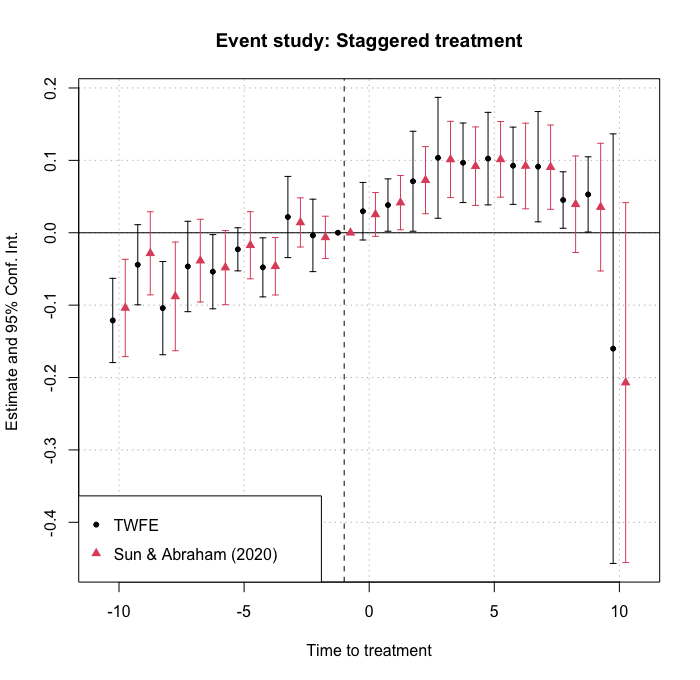
\includegraphics[width=\linewidth]{S-Inflow.png}
        \caption{Inflow}
        \label{22a}
    \end{subfigure}%
    \hfill
    % Subfigure (b) - Civilian Labor Force
    \begin{subfigure}{0.5\textwidth}
        \centering
        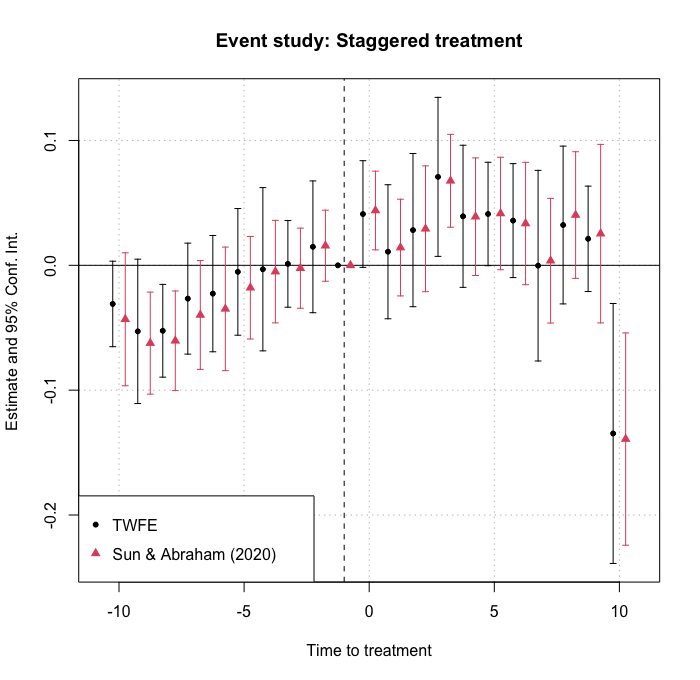
\includegraphics[width=\linewidth]{S-Outflow.png}
        \caption{Outflow}
        \label{22b}
    \end{subfigure}
    
    % Subfigure (c) - Unemployment Rate
    \begin{subfigure}{0.5\textwidth}
        \centering
        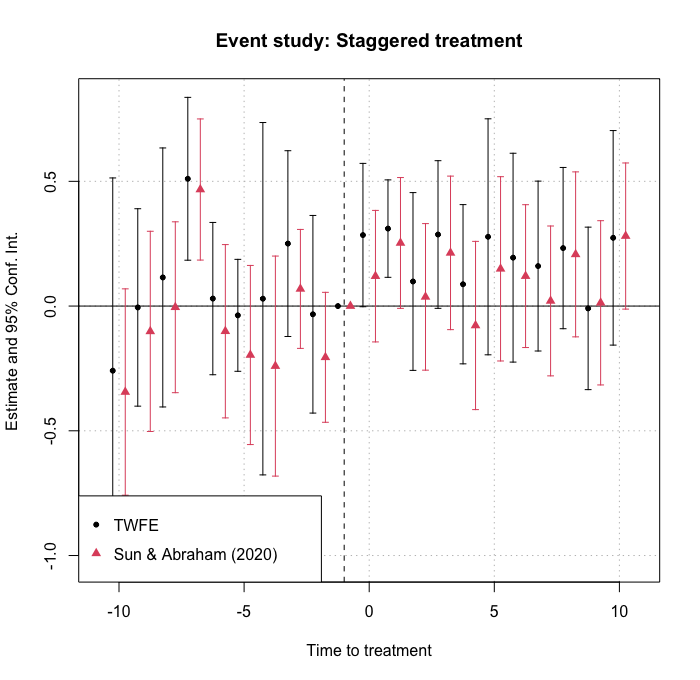
\includegraphics[width=\linewidth]{S-Netflow.png}
        \caption{Net Flow}
        \label{22c}
    \end{subfigure}%
    \hfill
    % Subfigure (d) - Republican Vote
    \begin{subfigure}{0.5\textwidth}
        \centering
        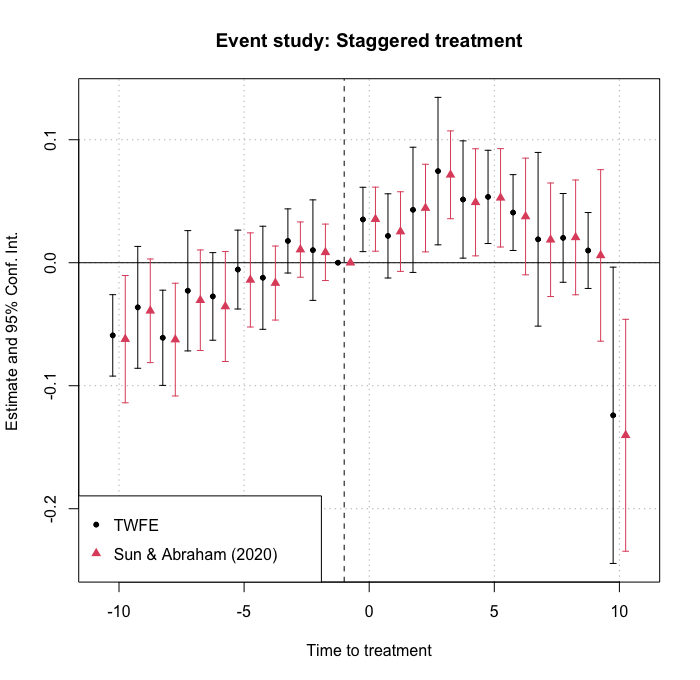
\includegraphics[width=\linewidth]{S-Grossflow.png}
        \caption{Gross Flow}
        \label{22d}
    \end{subfigure}
    
    % Caption and source
    \label{USflows}
    \caption*{\textit{Data Source:} IRS SOI Migration Flows, created by author}
\end{figure}

%%%%%%%%%%%%%%%%%%%%%%%%%%%%%%%%%%%%%%%%%%%%%%%%%%%%%%%%%%%%%%%%%%%%%%%%

\begin{figure}[H]
    \centering
    
    \caption{Severe Tornadoes' Impacts on Other Outcomes}
    \label{fig4}
    % Subfigure (a) - Median Housing Price
    \begin{subfigure}{0.5\textwidth}
        \centering
        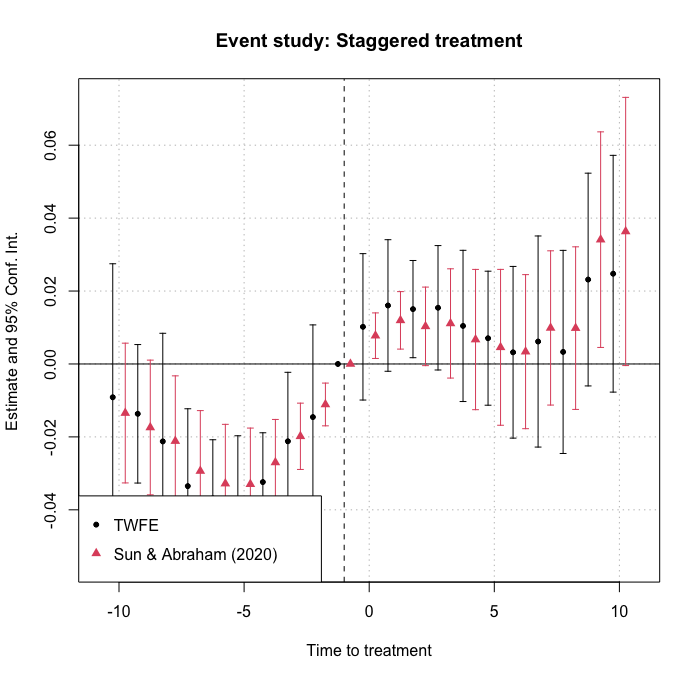
\includegraphics[width=\linewidth]{S-Housing.png}
        \caption{Median Housing Price}
        \label{22a}
    \end{subfigure}%
    \hfill
    % Subfigure (b) - Civilian Labor Force
    \begin{subfigure}{0.5\textwidth}
        \centering
        \includegraphics[width=\linewidth]{S-labor.png}
        \caption{Civilian Labor Force}
        \label{22b}
    \end{subfigure}
    
    % Subfigure (c) - Unemployment Rate
    \begin{subfigure}{0.5\textwidth}
        \centering
        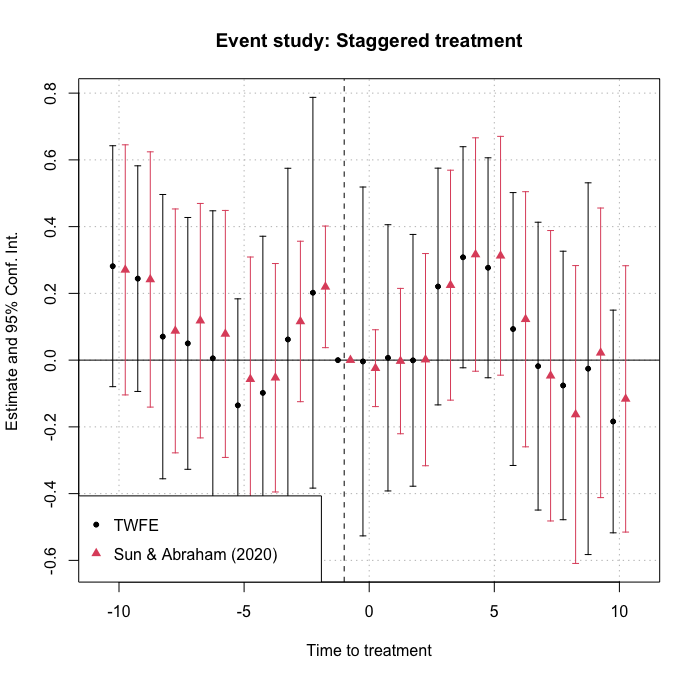
\includegraphics[width=\linewidth]{S-Unemployment.png}
        \caption{Unemployment Rate}
        \label{22c}
    \end{subfigure}%
    \hfill
    % Subfigure (d) - Republican Vote
    \begin{subfigure}{0.5\textwidth}
        \centering
        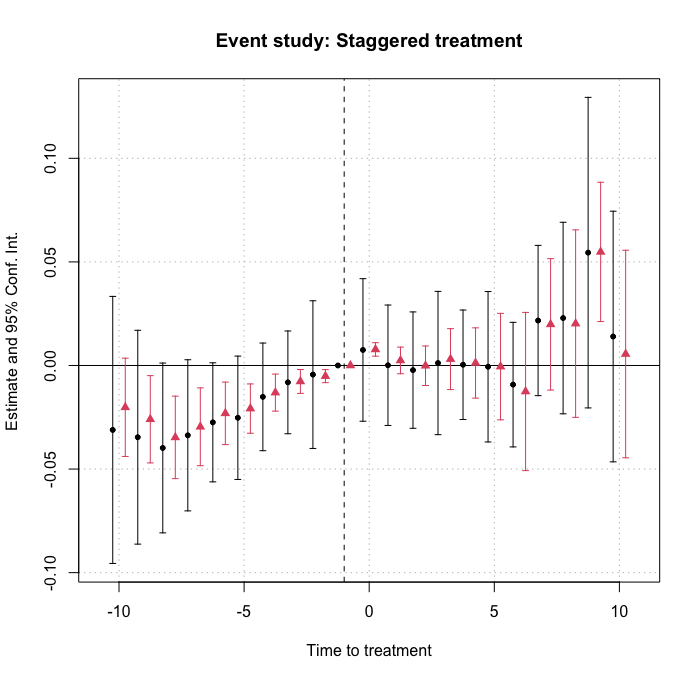
\includegraphics[width=\linewidth]{S-Republican.png}
        \caption{Republican Vote}
        \label{22d}
    \end{subfigure}
    
    % Caption and source
    \label{USflows}
    \caption*{\textit{Data Source:} U.S. Census, USDA, and Harvard Dataverse County Presidential
Return, created by author}
\end{figure}





 \begin{figure}
        \centering
        \caption{Severe Tornadoes' Impacts on Wage}
        \label{fig5}
        
        % Subfigure (a) - Inflow
        \begin{subfigure}[t]{0.5\linewidth}
            \centering
            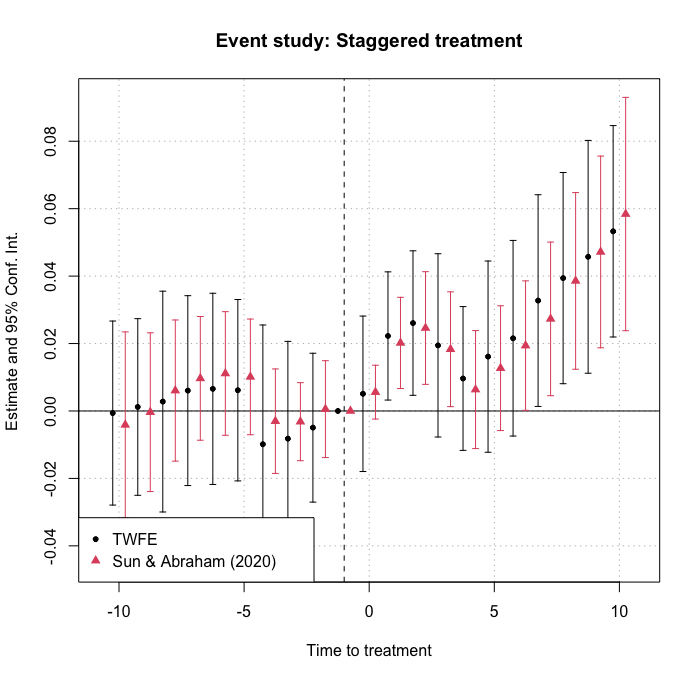
\includegraphics[width=\linewidth]{FinanceW.png}
            \caption{Wage: Financial Activities}
            \label{fig:inflow}
        \end{subfigure}
        \hfill
        % Subfigure (b) - Outflow
        \begin{subfigure}[t]{0.5\linewidth}
            \centering
            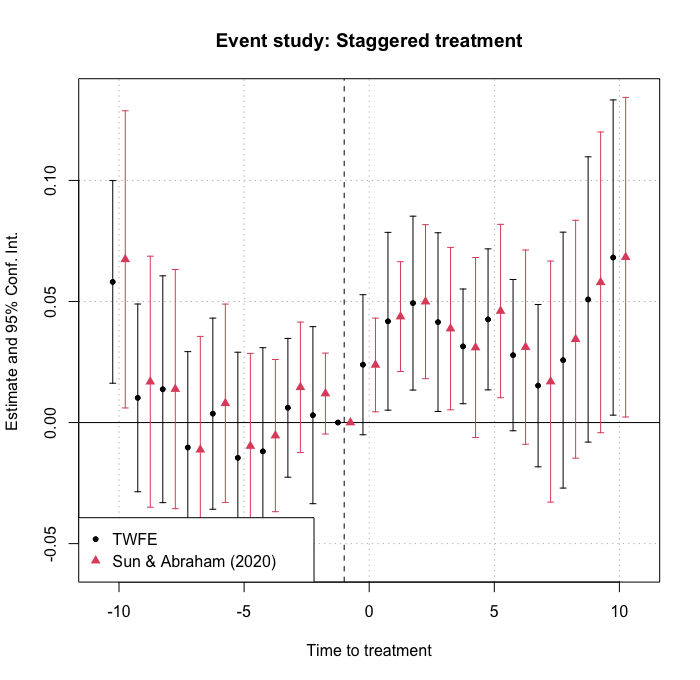
\includegraphics[width=\linewidth]{ProfessionalW.png}
            \caption{Wage: Professional and Business Services}
            \label{fig:outflow}
        \end{subfigure}
        
        % Caption and source
        \vspace{-10pt} % Adjust vertical spacing if necessary
        %\caption*{\textit{Data Source:} IRS SOI Migration Flows, created by author}
    \end{figure}

\end{document}
